\begin{figure}[t]
    \centering
    \begin{subfigure}[b]{0.49\textwidth}
        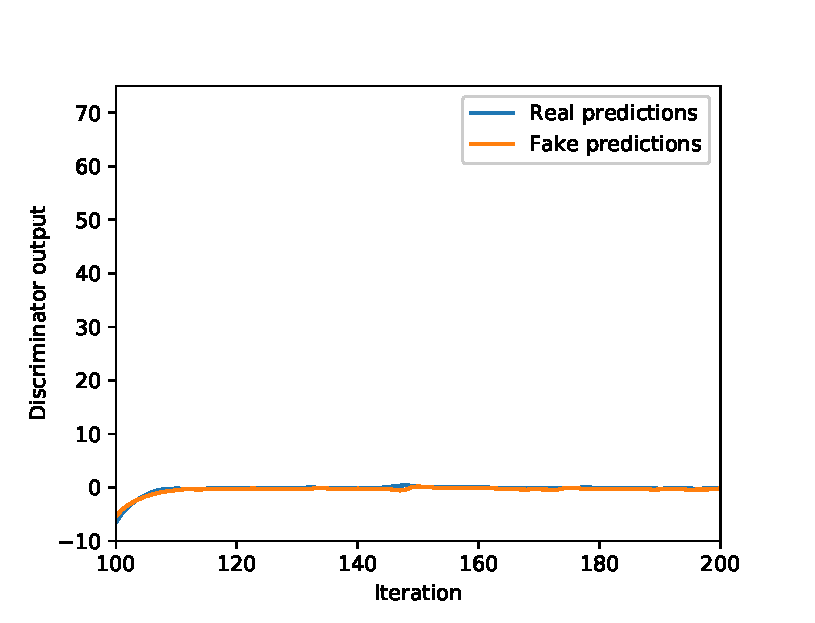
\includegraphics[width=\textwidth]{results/freezeInDG1_2.eps}
        \caption{Weight freezing in old layers}
        \label{fig:freezeInDG1}
    \end{subfigure}
    \begin{subfigure}[b]{0.49\textwidth}
        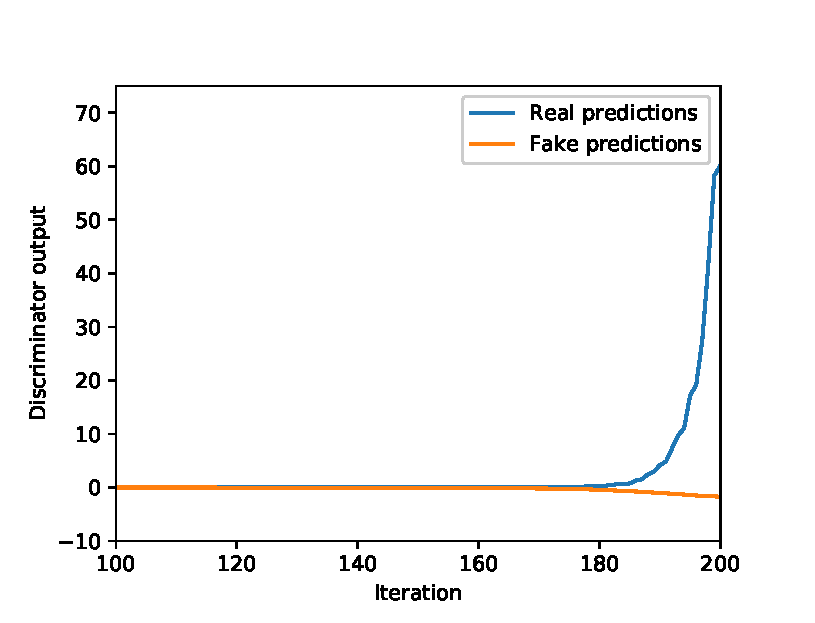
\includegraphics[width=\textwidth]{results/fadeInDG1_2.eps}
        \caption{Fade in new layers}
        \label{fig:freezeInDG2}
    \end{subfigure}
    \caption{Discriminator output on real and fake images during transition between 16x16 and 32x32 resolution images for the different transition strategies on the synthetic data set.}
    \label{fig:fadeVsFreeze}
\end{figure}

\begin{figure}[t]
    \centering
    \begin{subfigure}[b]{\textwidth}
        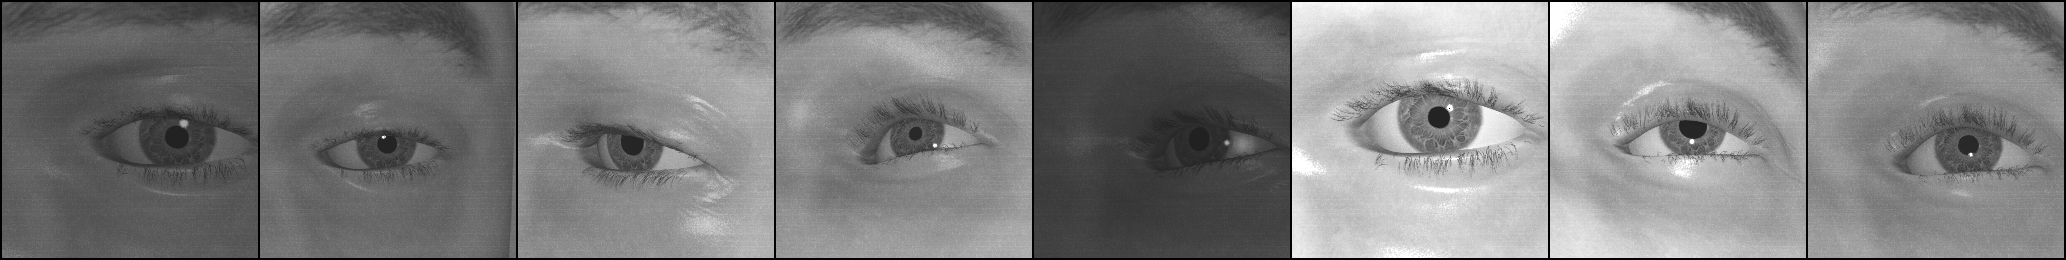
\includegraphics[width=\textwidth]{autoencoded/original.png}
        \caption{Original images}
        \label{fig:stuff}
    \end{subfigure}
    \begin{subfigure}[b]{\textwidth}
        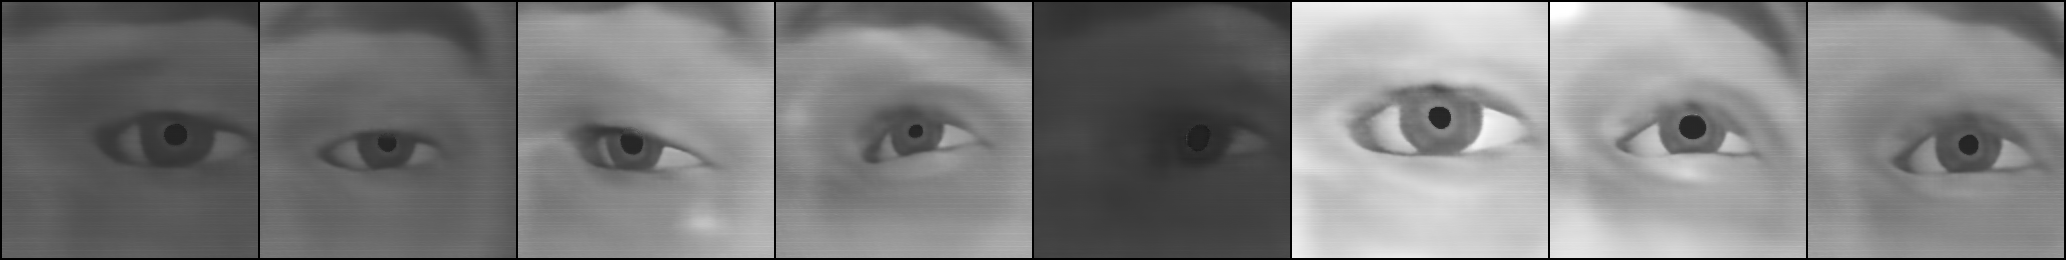
\includegraphics[width=\textwidth]{autoencoded/scaled_VAE_decoded.png}
        \caption{Decoded with VAE}
        \label{fig:stuff}
    \end{subfigure}
    \begin{subfigure}[b]{\textwidth}
        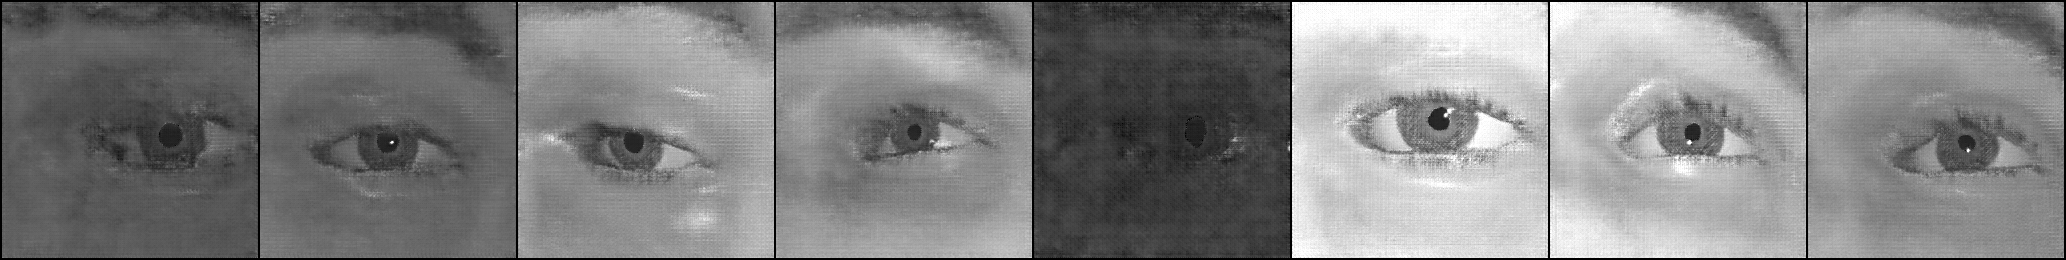
\includegraphics[width=\textwidth]{autoencoded/aegan_decoded.png}
        \caption{Decoded with \acrshort{aegan}}
        \label{fig:stuff}
    \end{subfigure}
    \caption{A batch of synthetic images, encoded and decoded by the encoder-decoder based methods.}
    \label{fig:autoencoders}
\end{figure}

\begin{figure}[t]
    \centering
    \begin{subfigure}[b]{\textwidth}
        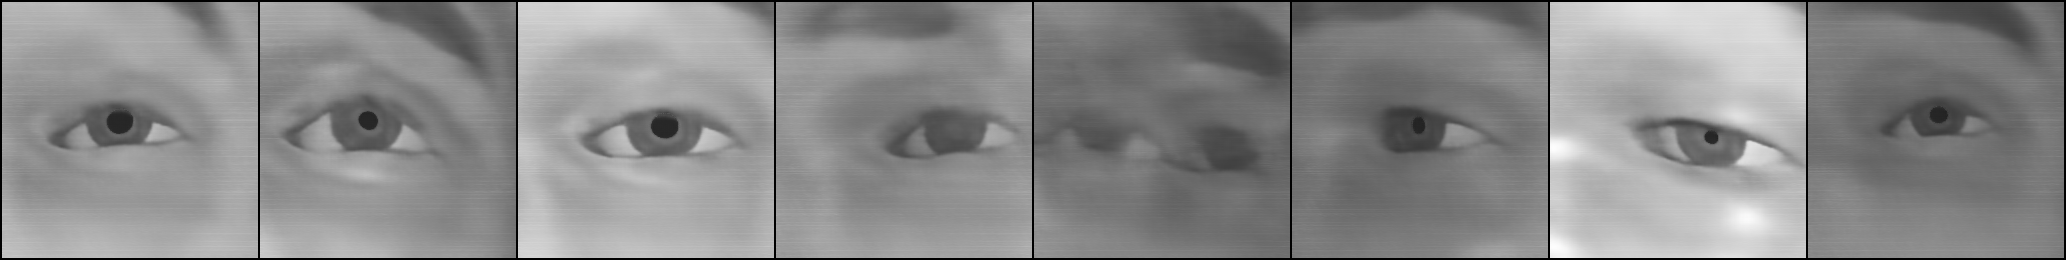
\includegraphics[width=\textwidth]{generated/vae_fake.png}
        \caption{Generated with VAE.}
        \label{fig:stuff}
    \end{subfigure}
    \begin{subfigure}[b]{\textwidth}
        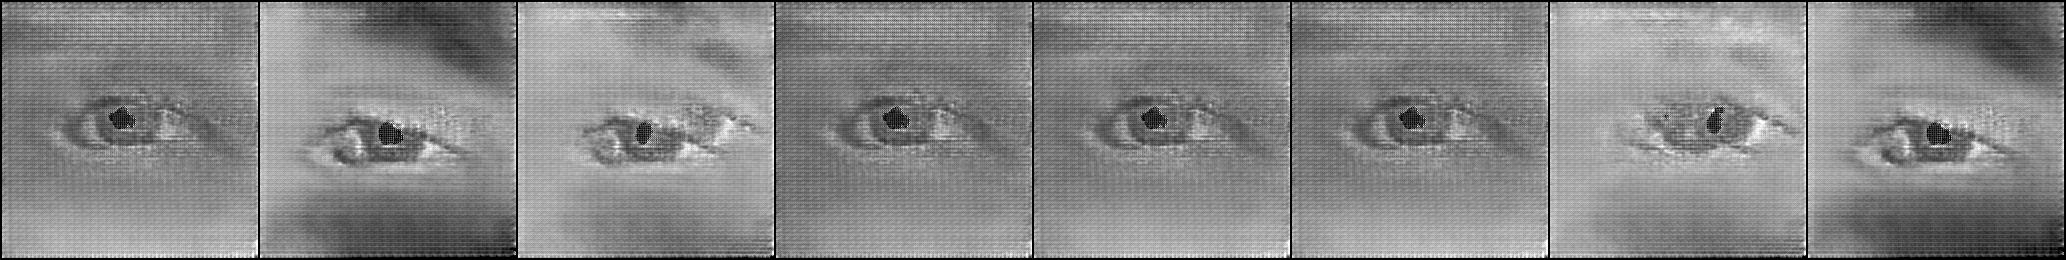
\includegraphics[width=\textwidth]{generated/wasserstein_fake.png}
        \caption{Generated with \acrshort{wgan}}
        \label{fig:stuff}
    \end{subfigure}
    \begin{subfigure}[b]{\textwidth}
        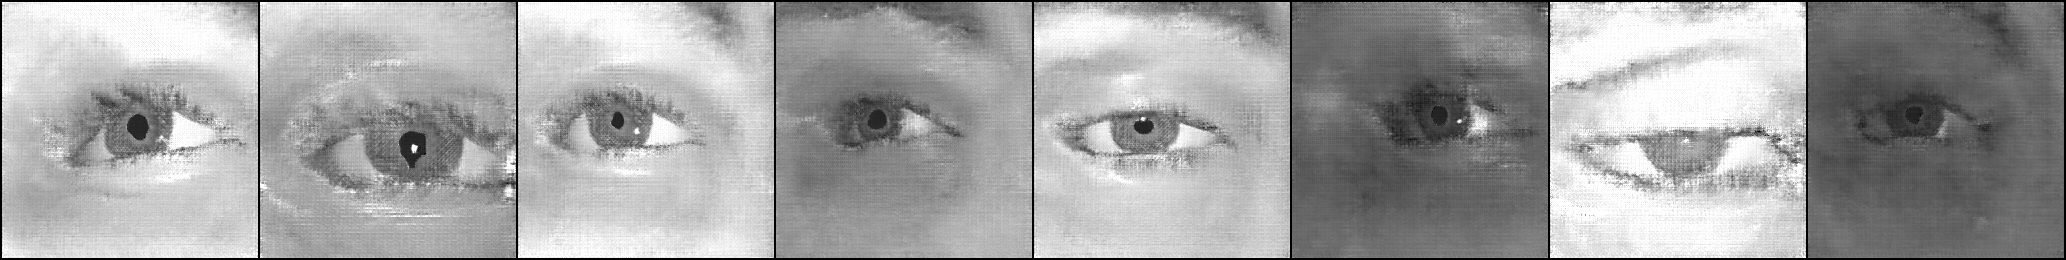
\includegraphics[width=\textwidth]{generated/aegan_fake.png}
        \caption{Generated with \acrshort{aegan}}
        \label{fig:stuff}
    \end{subfigure}
    \caption{Examples of a batch of generated images by the different models.}
    \label{fig:gans}
\end{figure}

\begin{table}[t]
    \centering
\caption{Jaccard distance between pupil regressor output and annotations for different sources of training data using synthesized data as the original data source. The leftmost columns indicate which data set the transformer was trained on. The test data used in \ref{subtab:on_real} is the original test set, whereas in \ref{subtab:on_fake} designated test sets were generated by the respective generative models.}
    \label{tab:quantitative_results}
    \begin{subtable}{0.9\textwidth}
        \begin{tabular}{|l|lll|}
            \cline{2-4}
            \multicolumn{1}{c|}{} & \multicolumn{3}{c|}{\textbf{Jaccard distance}} \\ \hline
            \textbf{Training data} & \acrshort{wgan} & VAE & \acrshort{aegan} \\ \hline
            Fake & \num{0.8132} & \num{0.159} & \textbf{\num{0.148}} \\
            Fake + real & \num{0.1219} & \textbf{\num{0.0944}} & \num{0.1032} \\
            \hline
            Real & \multicolumn{3}{c|}{\num{0.09607}} \\
            \hline
        \end{tabular}
        \caption{Tested on the real test data.}
        \label{subtab:on_real}
    \end{subtable}
    \begin{subtable}{0.9\textwidth}
        \begin{tabular}{|l|lll|}
            \cline{2-4}
            \multicolumn{1}{c|}{} & \multicolumn{3}{c|}{\textbf{Jaccard distance}} \\ \hline
            \textbf{Training data} & \acrshort{wgan} & VAE & \acrshort{aegan} \\ \hline
            Fake & \textbf{\num{4.82e-5}} & \num{0.0133} & \num{0.0491} \\ 
            Real & \num{0.1855} & \textbf{\num{0.0264}} & \num{0.1225} \\ 
            \hline
        \end{tabular}
        \caption{Test data generated by the generative models.}
        \label{subtab:on_fake}
        \end{subtable}
\end{table}

\begin{table}[t]
    \centering
    \caption{Jaccard distance between pupil regressor output and annotations for different sources of training data using models trained on real world data as original data. The structure and notation follows table \ref{tab:quantitative_results}.}
    \label{tab:quantitative_results_real}
    \begin{subtable}{0.9\textwidth}
        \begin{tabular}{|l|lll|}
            \cline{2-4}
            \multicolumn{1}{c|}{} & \multicolumn{3}{c|}{\textbf{Jaccard distance}} \\ \hline
            \textbf{Training data} & \acrshort{wgan} & VAE & \acrshort{aegan} \\ \hline
            Fake & \num{0.9966} & \num{0.3445} & \textbf{\num{0.2084}} \\
            Fake + real & \num{0.1215} & \textbf{\num{0.1151}} & \num{0.1221} \\
            \hline
            Real & \multicolumn{3}{c|}{\num{0.11456}} \\
            \hline
        \end{tabular}
        \caption{Tested on the real test data.}
    \end{subtable}
    \begin{subtable}{0.9\textwidth}
        \begin{tabular}{|l|lll|}
            \cline{2-4}
            \multicolumn{1}{c|}{} & \multicolumn{3}{c|}{\textbf{Jaccard distance}} \\ \hline
            \textbf{Training data} & \acrshort{wgan} & VAE & \acrshort{aegan} \\ \hline
            Fake & \textbf{\num{8.795e-6}} & \num{0.0284} & \num{0.0457} \\ 
            Real & \num{0.8798} & \num{0.1008} & \textbf{\num{0.0786}} \\ 
            \hline
        \end{tabular}
        \caption{Test data generated by the generative models.}
        \end{subtable}
\end{table}

\begin{table}[t]
    \centering
    \caption{Toy experiments on data augmentation}
    \label{tab:toy_experiments}
    \begin{subtable}{0.9\textwidth}
        \begin{tabular}{|l|ll|ll|ll|ll|}
            \cline{2-9}
            \multicolumn{1}{c|}{ } & \multicolumn{2}{c|}{Baseline} & \multicolumn{2}{c|}{WGAN} & \multicolumn{2}{c|}{VAE} & \multicolumn{2}{c|}{AEGAN} \\ \hline
            \textbf{Data set} & Mean & Std & Mean & Std & Mean & Std & Mean & Std \\ \hline
            Iris & \num{0.19751941} & \num{0.010727016} & \num{0.216506} & \num{0.0261355455} & \num{0.2040766} & \num{0.0093358} & \num{0.1780217} & \num{0.0084796728} \\
            \hline
        \end{tabular}
    \end{subtable}
    \begin{subtable}{0.9\textwidth}
        \begin{tabular}{|l|lll|l|l|}
            \cline{2-6}
            \multicolumn{1}{c|}{} & Baseline 100 & Baseline 200 & Baseline 400 & VAE & AEGAN \\ \hline
            Error rate ($\%$) & \num{0.90} & \num{1.02} & \num{0.87} & \num{1.33} & \textbf{\num{0.86}} \\ \hline
        \end{tabular}
    \end{subtable}
\end{table}


%\begin{table}[t]
%    \centering
%    \caption{Jaccard distance between pupil regressor output and annotations for different sources of training data using models trained on real world data as original data. The structure and notation follows table \ref{tab:quantitative_results}.}
%    \label{tab:quantitative_results_real}
%    \begin{tabular}{|ll|lll|lll|}
%        \cline{3-8}
%        \multicolumn{2}{c}{ } & \multicolumn{3}{|c|}{JD} & \multicolumn{3}{c|}{RD ($\%$)} \\ \hline
%        \textbf{Train} & \textbf{Test} & \acrshort{wgan} & VAE & \acrshort{aegan} & \acrshort{wgan} & VAE & \acrshort{aegan} \\ \hline
%        F & R & \num{0.9966} & \num{0.3445} & \textbf{\num{0.2084}} & \num{869.9} & \num{303.8} & \textbf{\num{183.8}} \\
%        F & F & \textbf{\num{8.795e-6}} & \num{0.0284} & \num{0.0457} & \textbf{\num{0.00768}} & \num{25.0} & \num{40.3} \\ 
%        R & F & \num{0.8798} & \num{0.1008} & \textbf{\num{0.0786}} & \num{768.0} & \num{88.9} & \textbf{\num{62.3}} \\ 
%        F + R & R & \num{0.1215} & \textbf{\num{0.1151}} & \num{0.1221} & \num{106.1} & \textbf{\num{101.5}} & \num{107.7} \\ 
%        \hline
%        R & R & \multicolumn{3}{c|}{\num{0.11456}} & \multicolumn{3}{c|}{100} \\
%        \hline
%    \end{tabular}
%\end{table}

%\begin{table}[t]
%    \centering
%    \caption{Jaccard distance between pupil regressor output and annotations on synthetic data}
%    \label{tab:quantitative_results}
%    \begin{tabular}{l|l|l}
%    \hline
%    %\multicolumn{3}{c}{Generator}           \\ 
%    Training data type      & MEE synthetic data  & MEE Accuracy real data \\ \hline
%    Original data           & $\sim$ 0.3 & 1.1     \\
%    VAE                     & $\sim$ 1.7 & 1.9     \\
%    VAE + original data     & 0.3 (guess) & 134     \\
%    %PGAN                    & 5.4 (pessimistic guess) & 134     \\
%    %PGAN + original data    & 0.3 (optimistic guess) & 134     \\
%    \acrshort{aegan}                   & 0.3 (optimistic guess) & 134     \\
%    \acrshort{aegan} + original data   & 0.3 (guess) & 134     \\
%    \end{tabular}
%\end{table}

A set of exploratory experiments were conducted for the different proposed methods to find settings where the methods succeed at producing visually pleasing data. Due to the unstable nature of \acrshort{gans} and the limited available resources in this project, most of \todoproofread{the} experiments based on \acrshort{gans} failed to do this. The few successful models also turned out to be highly sensitive to changes in network architecture, hyperparameters or training setup leaving a lo\st{o}t of room for improvement and further investigations. 

Of the tested methods, only the \acrshort{vae} and \acrshort{aegan} were capable of producing data with some visual resemblance to the original data. The Wasserstein GAN suffered from severe mode collapse and training instability thereby resulting in only failures.

The progressive \acrshort{gan} produced promising results on the initial stages with highly downsampled data. However the proposed fade-in procedure failed, forcing the model to re-learn everything from scratch at each stage of training. At the lower stages the model was capable of recovering after the fade-in but not on the full resolution stage, resulting in behaviour similar to the normal \acrshort{wgan}. 

To circumvent the fade-in issues of the progressive \acrshort{gan} an alternative freeze-in method of introducing the layers was tested. This approach views the introduction of the new layers as a transfer learning problem and freezes all but the newly introduced weights for a number of iterations. The method resembles gradual tuning for transfer learning \parencite{montone2017gradual}. The discriminator output of the progressive \acrshort{gan} during fade-in and freeze-in is illustrated in figure \ref{fig:fadeVsFreeze}. In this figure one can see that the freeze-in strategy results in a more stable transition between the stages. However this strategy requires the adversarial game between the last layers of the generator and the first layers of the discriminator to be balanced for all transitions which was observed not to be the case, which is why the progressive \acrshort{gan} is not featured in any further evaluation.

\section{Qualitative Results}
Figure \ref{fig:autoencoders} shows a batch of images, together with the same batch after being encoded and decoded by both a \acrshort{vae} and an \acrshort{aegan}. From this figure it is clear that both of these methods have managed to learn to capture the main aspects of the full data distribution. Both methods display varying illuminance levels, pupil dilations, different reflections and eyelid openness. However it is common for both methods to fail to capture the original information in some of these such as pupil dilation. Even though the methods display a clear variance in pupil dilation, the reconstructed dilation does not always correspond to the original pupil size.

The single most striking observation to emerge from comparing these images is the level of details captured by the \acrshort{aegan}. Unlike the \acrshort{vae}, the \acrshort{aegan} learned to produce glints and sharp eyelashes. It is also interesting to note that the glints are sometimes correctly positioned which due to the structure of deep convolutional neural networs \todoproofread{networks} is not easily learned. However in many cases it can be seen that the glints are poorly placed.

Decoding images from a learned posterior is not the same as generating new images from the prior distribution. Examples of generated images from a $\mathcal{N}(0, 1)$ distribution are shown in figure \ref{fig:gans}. In this case the \acrshort{wgan} is also featured as it allows sampling new data. 

What stands out in this figure after observing the decoded images is the \acrshort{vae} images, which sometimes looks decent as before but in some cases looks more artistic than realistic \todocomment{Might be stating the obvious, but you could mension that the images appear blurred or are missing high-frequency details}. Except for this observation, it is also clear from the figure that the \acrshort{wgan} suffered from severe mode collapse wereas the \acrshort{aegan} managed to capture both a good variance and visually pleasing quality of some of the samples even though some artefacts easily can be spotted in most images.

% However, failing to position the glints correctly causes the \acrshort{gan} objective and the autoencoder loss to operate in different directions, as the autoencoder loss will penalize the existance of wrongly placed glints causing the model to generate more modest and non-realistic glints which in turn will be penalized by the \acrshort{gan}.  <- Diskussionsmaterial ? 

% ...
%A comparison between a VAE and the autoencoder part of an \acrshort{aegan} is shown in figure <Referera till figur>. It is clear from this illustration that the simultaneous training of the GAN caused the autoencoder to generate more visually pleasing samples.

\section{Quantitative Results}
For the quantitative evaluation the default transofrmer was trained to generate segmentation maps from images of eyes. The images in this context can be directly from one of the data sets as well as from a generative model trained on one of these data sets. In the first case the images are denoted as "real" images, and in the second case they are denoted as "fake". 

The difference between the predicted segmentation map and the original was defined as the Jaccard Distance, defined as
\begin{equation}
    D_{Jaccard}(X, Y) = 1 - \frac{X \cap Y}{X \cup Y},
    \label{eq:jaccard}
\end{equation}
where the sets $X$ and $Y$ is the set of activated pixles in the respective segmentation map, which corresponds to the set of $1$:s \todoproofread{I think this colon is a Swedish thing, remove} for the real annotations. Any segmentation map generated by a neural network may include any floating point value for each pixel. These values were therefore rounded to produce a binary segmentation map. In this evaluation there exists images without pupils in some images, this results in computing the Jaccard distance between the empty set. To solve this all sets implicitly contain an extra element common to all sets. This can easily be computed as it only requires adding $1$ to the denominator and numerator in the fraction in (\ref{eq:jaccard}).

The Jaccard distances for segmentation maps produced by transformers trained and tested on different data sets \st{is} \todoproofread{are} shown in table \ref{tab:quantitative_results} for the models trained on synthetic data and in table \ref{tab:quantitative_results_real} for the models trained on the real world data. The most important results in both of these tables is the first row which roughly corresponds to the direct usability of the generated data. In both cases, the \acrshort{aegan} performed best for this measure indicating as already qualitatively observed that the \acrshort{aegan} produced the best data sets. Another interesting finding is that training on both generated data and real world data did not increase the perfromance on real data for any of the cases except the \acrshort{vae} on synthetic data, where the test distance were slightly lower thant the original test distance. \todocomment{I think this sentence can be a little unclear, how about: "training on both generated data and real world data did not manage to outperform training on real data alone for all cases except the VAE on synthetic data"}

%\section{The effect of sampling bias}  % - borde skriva om detta i metod-delen också
%TODO: Undersök om AEGANv2 kan augmentera MNIST med förbättrat resultat. Kontrastera resultat mot v1 med tolkningen att v2 är mindre påverkad av sampling-bias. Samma sak bör göras med VAE. Ifall posterior-augmentering är bättre än vanlig så bör uppskalade experiment också genomföras.

\section{Augmenting data for classification}
% TODO: Formulera om Iris som klassificeringsprblem

In the case of discrete classification there is no obvious method for concatenating data with the annotations. On the other hand it is sensible to assume that a small peturbation of an image does not alter the class label. With this assumption the autoencoder-based methods can still be used for data augmentation. Instead of sampling the latent points for the new data from the prior distribution $P(Z)$, they are sampled from the posterior $P(Z|X=x)$ yielding new data points. This procedure was tested on the MNIST dataset, the results are illustrated in table \ref{tab:toy_experiments}. \todocomment{This prargraph feels like it came out of nowhere, \bf{edit}: I see that it is a work in progress.}

%In table \ref{tab:quantitative_results}

%Quantitative results can be seen in table \ref{tab:quantitative_results}.



%\begin{table}[t]
%    \centering
%    \caption{Number of iterations of training for the different algorithms}
%    \label{tab:quantitative_results}
%    \begin{tabular}{l|l|l}
%    \hline
%    %\multicolumn{3}{c}{Generator}           \\ 
%    Training data type      & Synthetic data  & Real data \\ \hline
%    VAE                     & 560000 & 560000 \\
%    PGAN                    & idk & idk     \\
%    \acrshort{aegan}                   & 520000 & 840000   \\
%    \end{tabular}
%\end{table}

%TODO: Visa kapacitet/overfitting på samma dataset, visa att genererad data är konsistent och har bra annoteringar!

%<<Lägg till ett par histogram här.>>

%<<Figur med referensbatch och decoded för VAE, AE och \acrshort{aegan}. Inkludera L1-fel för samtliga rekonstruktioner>>


